\documentclass[tikz,border=2pt]{standalone}
\usepackage{amsmath,amssymb}
\usepackage{pgfplots}
\pgfplotsset{compat=1.18}
\usetikzlibrary{arrows.meta}
\begin{document}
% Retention d = 1, payment (x-d)_+ is convex. Y in {0,2} with probability 1/2 each pays 0 or 1, so
% E[(Y-1)_+] = 0.5 (chord midpoint); X = 1 = E[Y] pays (1-1)_+ = 0. Jensen: the constant has no larger expected excess.
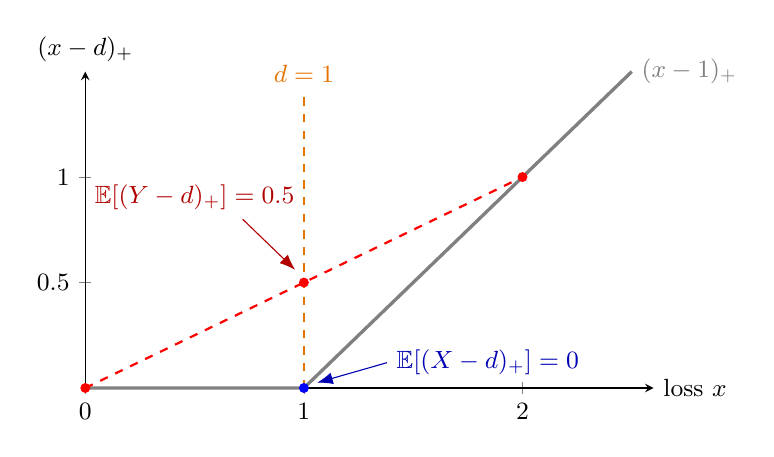
\begin{tikzpicture}[font=\small, >={Latex[length=2mm]}]
  \begin{axis}[
    axis lines=left, xmin=0, xmax=2.6, ymin=0, ymax=1.5,
    xtick={0,1,2}, ytick={0.5,1},
    xlabel={loss $x$}, ylabel={$(x-d)_+$},
    xlabel style={at={(axis description cs:1,0)}, anchor=west},
    ylabel style={rotate=-90, at={(axis description cs:0,1)}, anchor=south},
    width=8.8cm, height=5.6cm, clip=false
    ]
    \draw[orange!90!black, thick, dashed] (axis cs:1,0) -- (axis cs:1,1.4);
    \node[orange!90!black, anchor=south] at (axis cs:1,1.4) {$d=1$};
    \addplot[gray, very thick] coordinates {(0,0) (1,0) (2.5,1.5)};
    \node[gray, anchor=west] at (axis cs:2.5,1.5) {$(x-1)_+$};
    % Y: chord between its two outcomes
    \draw[red, thick, dashed] (axis cs:0,0) -- (axis cs:2,1);
    \fill[red] (axis cs:0,0) circle (1.8pt);
    \fill[red] (axis cs:2,1) circle (1.8pt);
    \fill[red] (axis cs:1,0.5) circle (1.8pt);
    \node[red!70!black, anchor=south] at (axis cs:0.5,0.8) {$\mathbb E[(Y-d)_+]=0.5$};
    \draw[red!70!black, ->] (axis cs:0.72,0.8) -- (axis cs:0.96,0.56);
    % X: the constant 1
    \fill[blue] (axis cs:1,0) circle (1.8pt);
    \draw[blue!70!black, ->] (axis cs:1.38,0.12) -- (axis cs:1.06,0.025);
    \node[blue!70!black, anchor=west] at (axis cs:1.38,0.12) {$\mathbb E[(X-d)_+]=0$};
  \end{axis}
\end{tikzpicture}
\end{document}
